\section{Traffic Light Controller simulation}
\label{sec:casestudy}
In order to assess the usability and practicality of UML State Machines and RAOES, we consider a simplified Traffic Light Controller (TLC) system as a case study, which is extracted from \cite{katz2005contemporary}.
TLC controls an intersection of a busy highway and a little-used farm-way.

%\ti{" Detectors are placed along the farmroad to raise the signal C as long as a vehicle is waiting to cross the highway. The traffic light controller should operate as follows. As long as no vehicle is detected on the farmroad, the lights should remain green in the highway direction. If a vehicle is detected on the farmroad, the highway lights should change from yellow to red, allowing the farmroad lights to become green. The farmroad lights stay green only as long as a vehicle is detected on the farmroad and never longer than a set interval to allow the traffic to flow along the highway. If these conditions are met, the farmroad lights change from green to yellow to red, allowing the highway lights to return to green. Even if vehicles are waiting to cross the highway, the highway should remain green for a set interval"}.
The system is shown in Fig. \ref{fig:casestudy}.

\begin{figure}
	\centering
	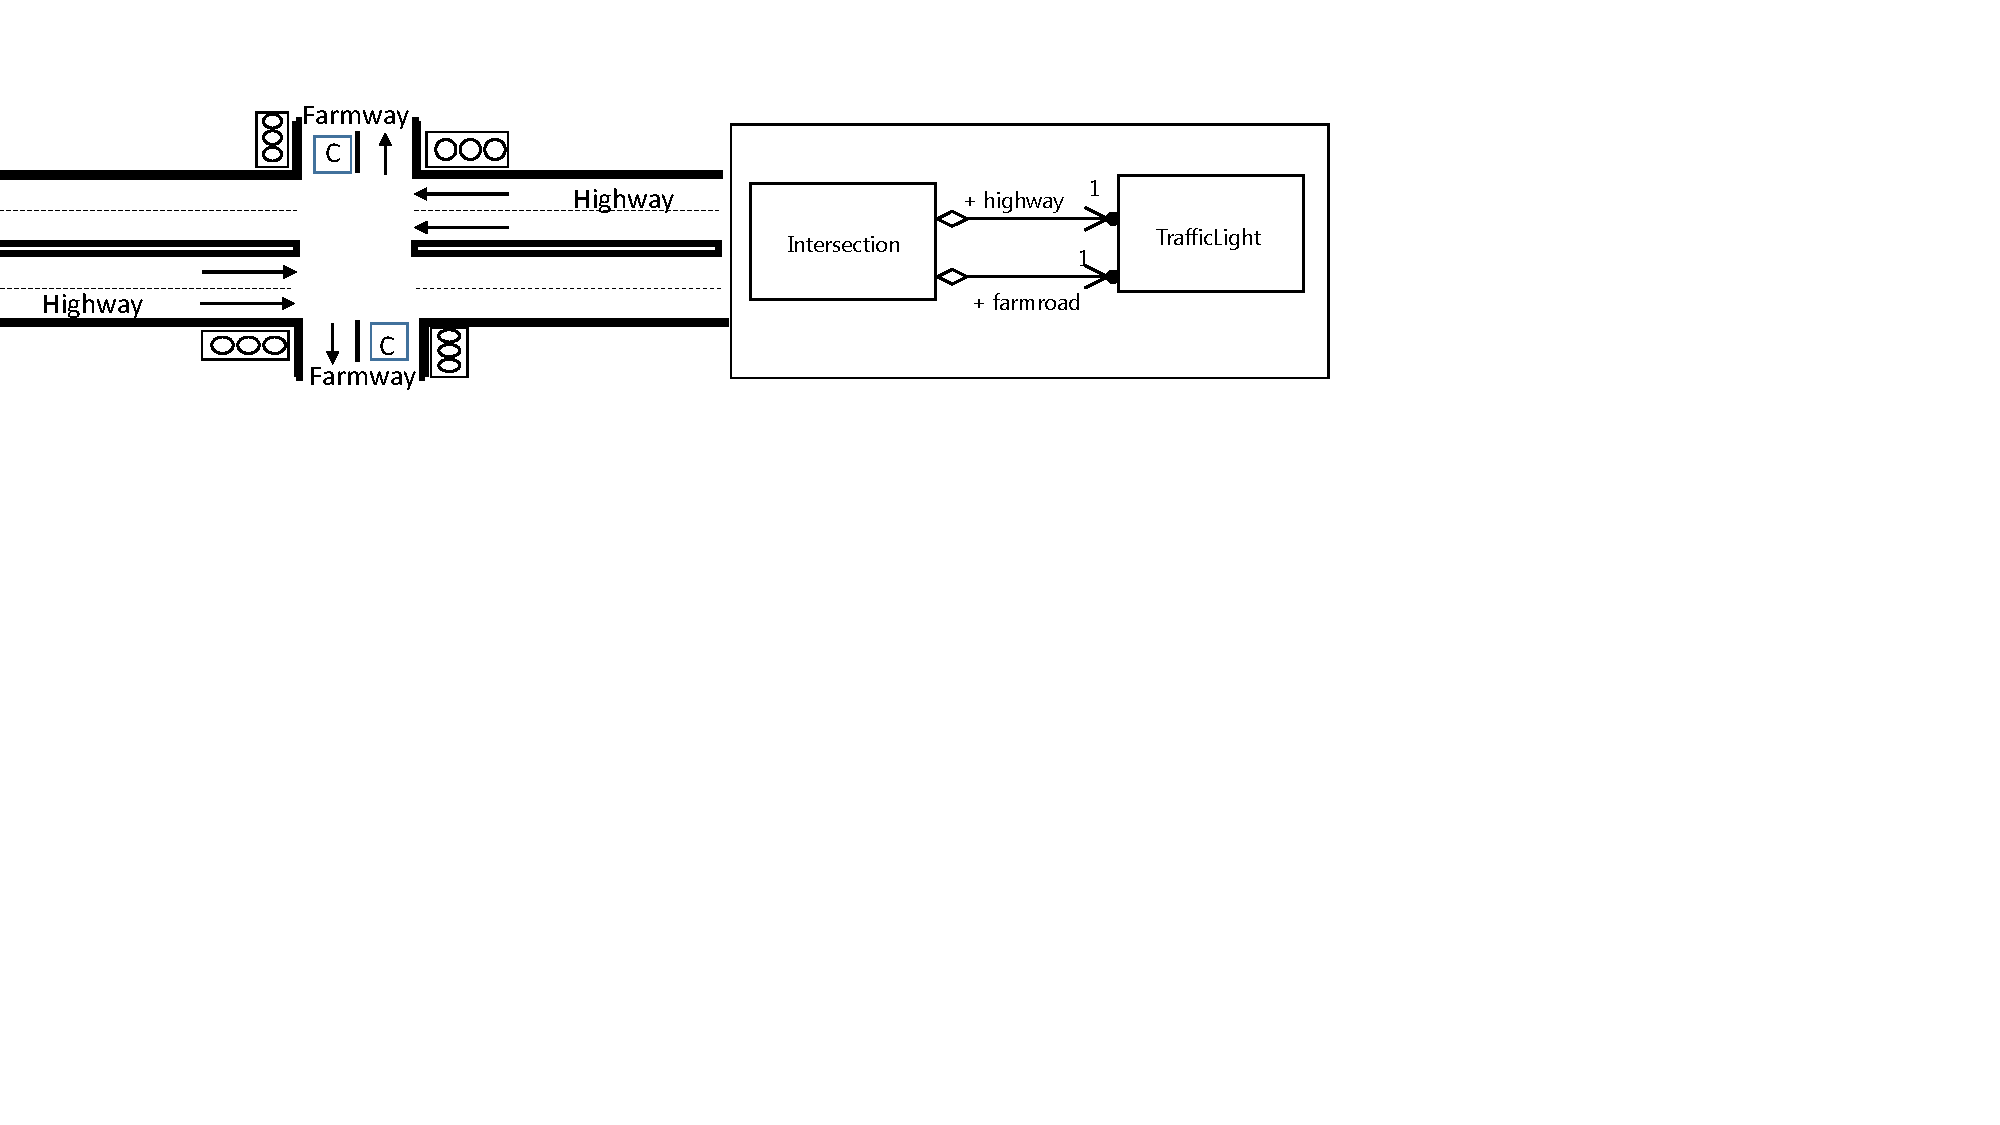
\includegraphics[clip, trim=0.6cm 10.4cm 10.9cm 0cm, width=1.0\columnwidth]{figures/casestudy}
	\caption{Traffic Light Controller (left) and its class diagram (right).} 
	\label{fig:casestudy}
\end{figure}





To apply RAOES, a software architect and a programmer participated to the development.
The class system design is similar to the object-oriented one presented in \cite{trafficlight}.
Each class's behavior is described by USMs.
However, the state machine describing the behavior of \ttt{Intersection} in our design is invented by two ways utilizing \ttt{ChangeEvent}s and the deference of events in USM, respectively.


The design of behaviors of \ttt{Intersection} and \ttt{TrafficLight} is shown in Fig. \ref{fig:casestudystatemachine} (left and right, respectively).
It is worth noting that the states of \ttt{IntersectionStateMachine}, except \ttt{FarmwayOpen} are composite.
The details of \ttt{SwitchingHighwayToFarmroad} and \ttt{SwitchingFarmroadToHighway} are actually shown on the yasmine site \cite{farmroadexample}.

\begin{figure}
	\centering
	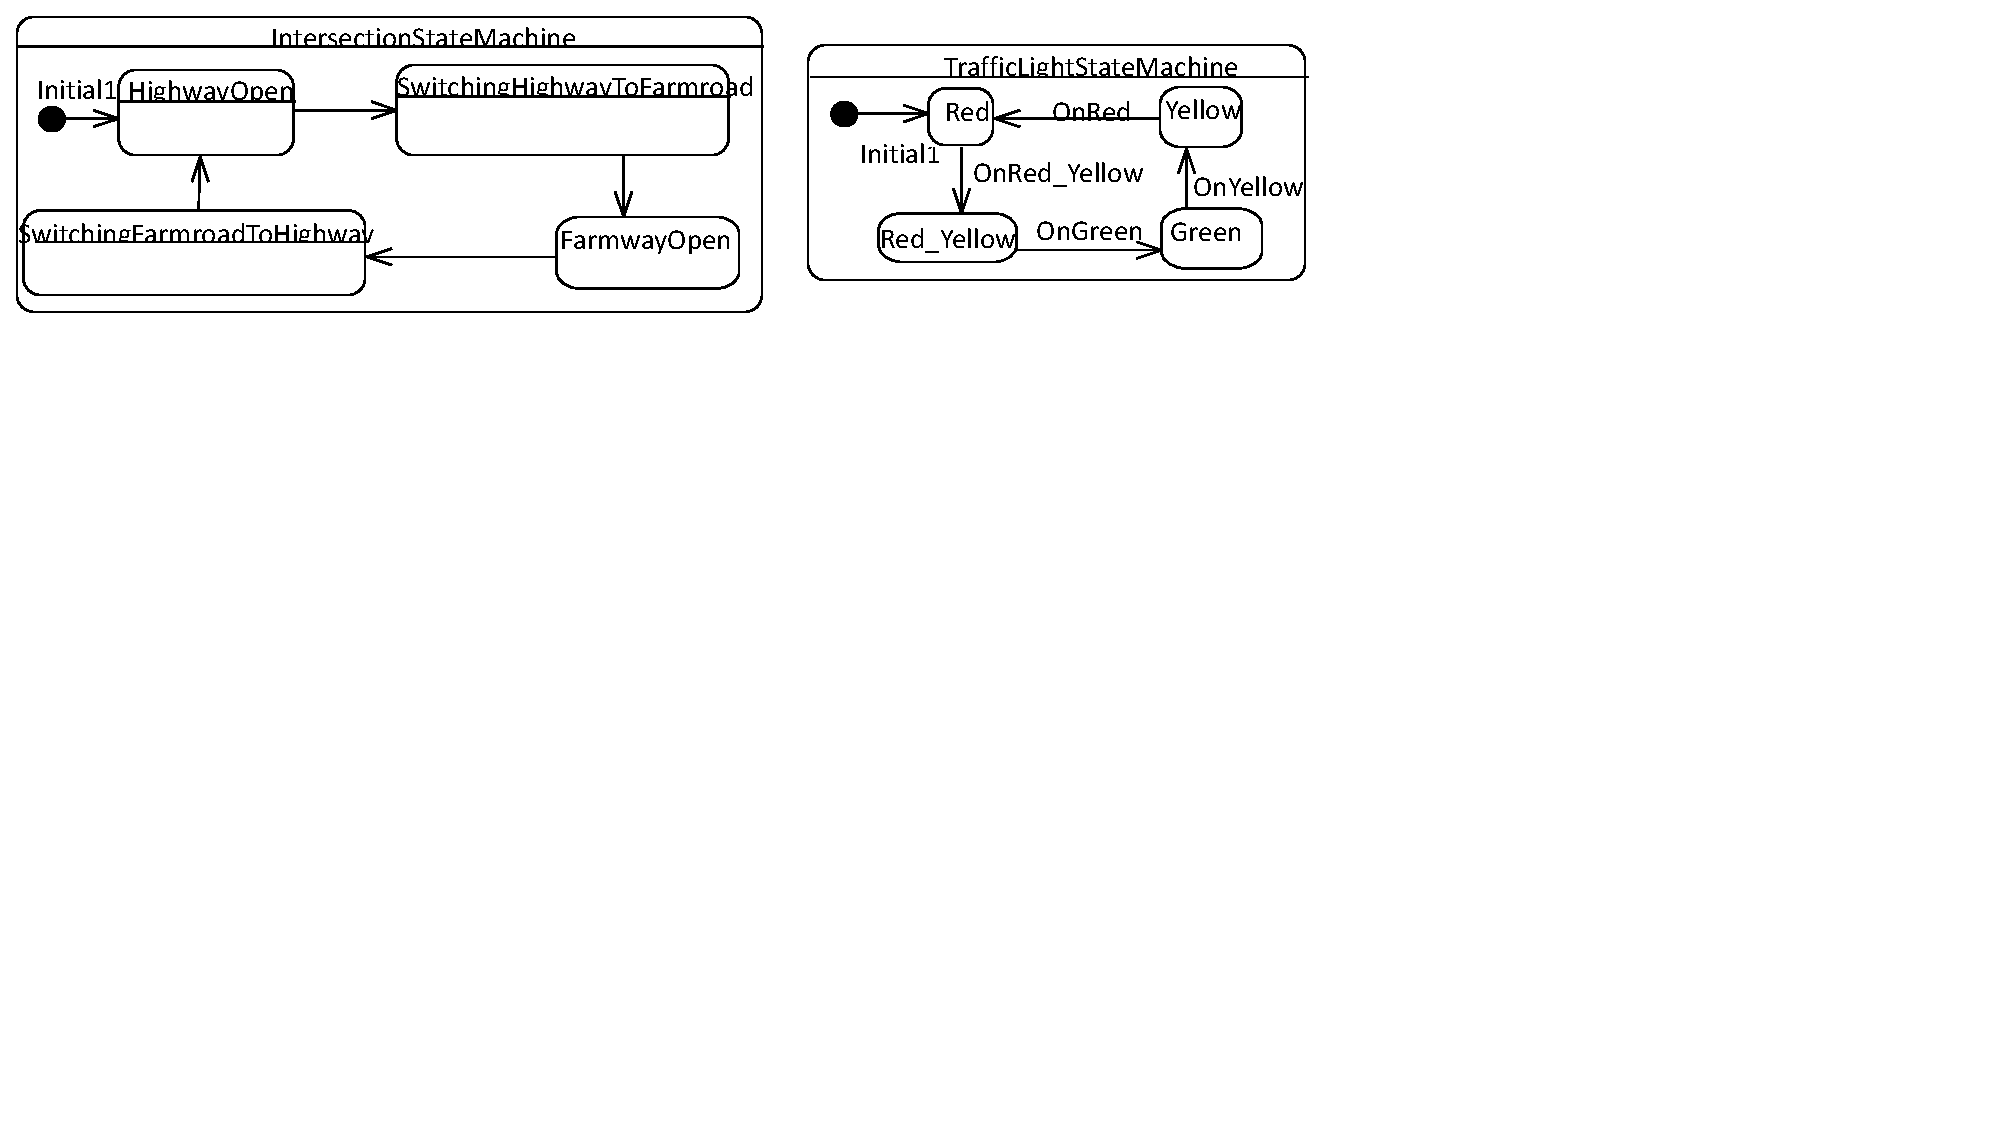
\includegraphics[clip, trim=0.2cm 13.6cm 10.9cm 0.2cm, width=1.0\columnwidth]{figures/casestudystatemachine}
	\caption{State machines for describing the behavior of Intersection (left) and TrafficLight (right)} 
	\label{fig:casestudystatemachine}
\end{figure}


%alternative design for the HighwayOpen composite state
The requirements for switching from the state \ttt{HighwayOpen} to \ttt{SwitchingHighwayToFarmroad} are: (1) a minimum time for the highway open is elapsed; and (2) the sensors signal.
Fig. \ref{fig:highwayopenalternatives} (b) and (d) shows the alternative designs for the composite state \ttt{HighwayOpen}, and Fig. \ref{fig:highwayopenalternatives} (a) and (c) displays their respective version written in C++ front-end.
The design in ((a) and (b)) uses a \ttt{TimeEvent} and the event deference.
Specifically, when \ttt{HighwayOpen} becomes active, its active sub-state remains \ttt{WaitingForHighwayMinimum} as long as the minimum time.
If the a signal event is emitted from the detector, the event is delayed until the active sub-state becomes \ttt{MinimumTimeElapsed}.
The event is then processed to finish the execution of \ttt{HighwayOpen} and active the farmway.

The other design utilizes a \ttt{ChangeEvent} for triggering the switching the active sub-state of \ttt{HighwayOpen} from \ttt{WaitForPreconditions} to a final state. 
The expression associated with the change event changes from false to true once two flags \ttt{timeFlag} (for \ti{minimum time elapsed}) and \ttt{detectFlag} (for \ti{vehicle detected on the farmroad}) are set. 
\ttt{timeFlag} is set by executing the effect \ttt{setTime} of the internal transition of \ttt{WaitForPreconditions} triggered by the \ttt{TE\_MIN} time event. 
And \ttt{detectFlag} is set by the method \ttt{setDetect} once a \ttt{DetectorOn} event occurs to trigger another internal transition of \ttt{WaitForPreconditions}.
\begin{figure}
	\centering
	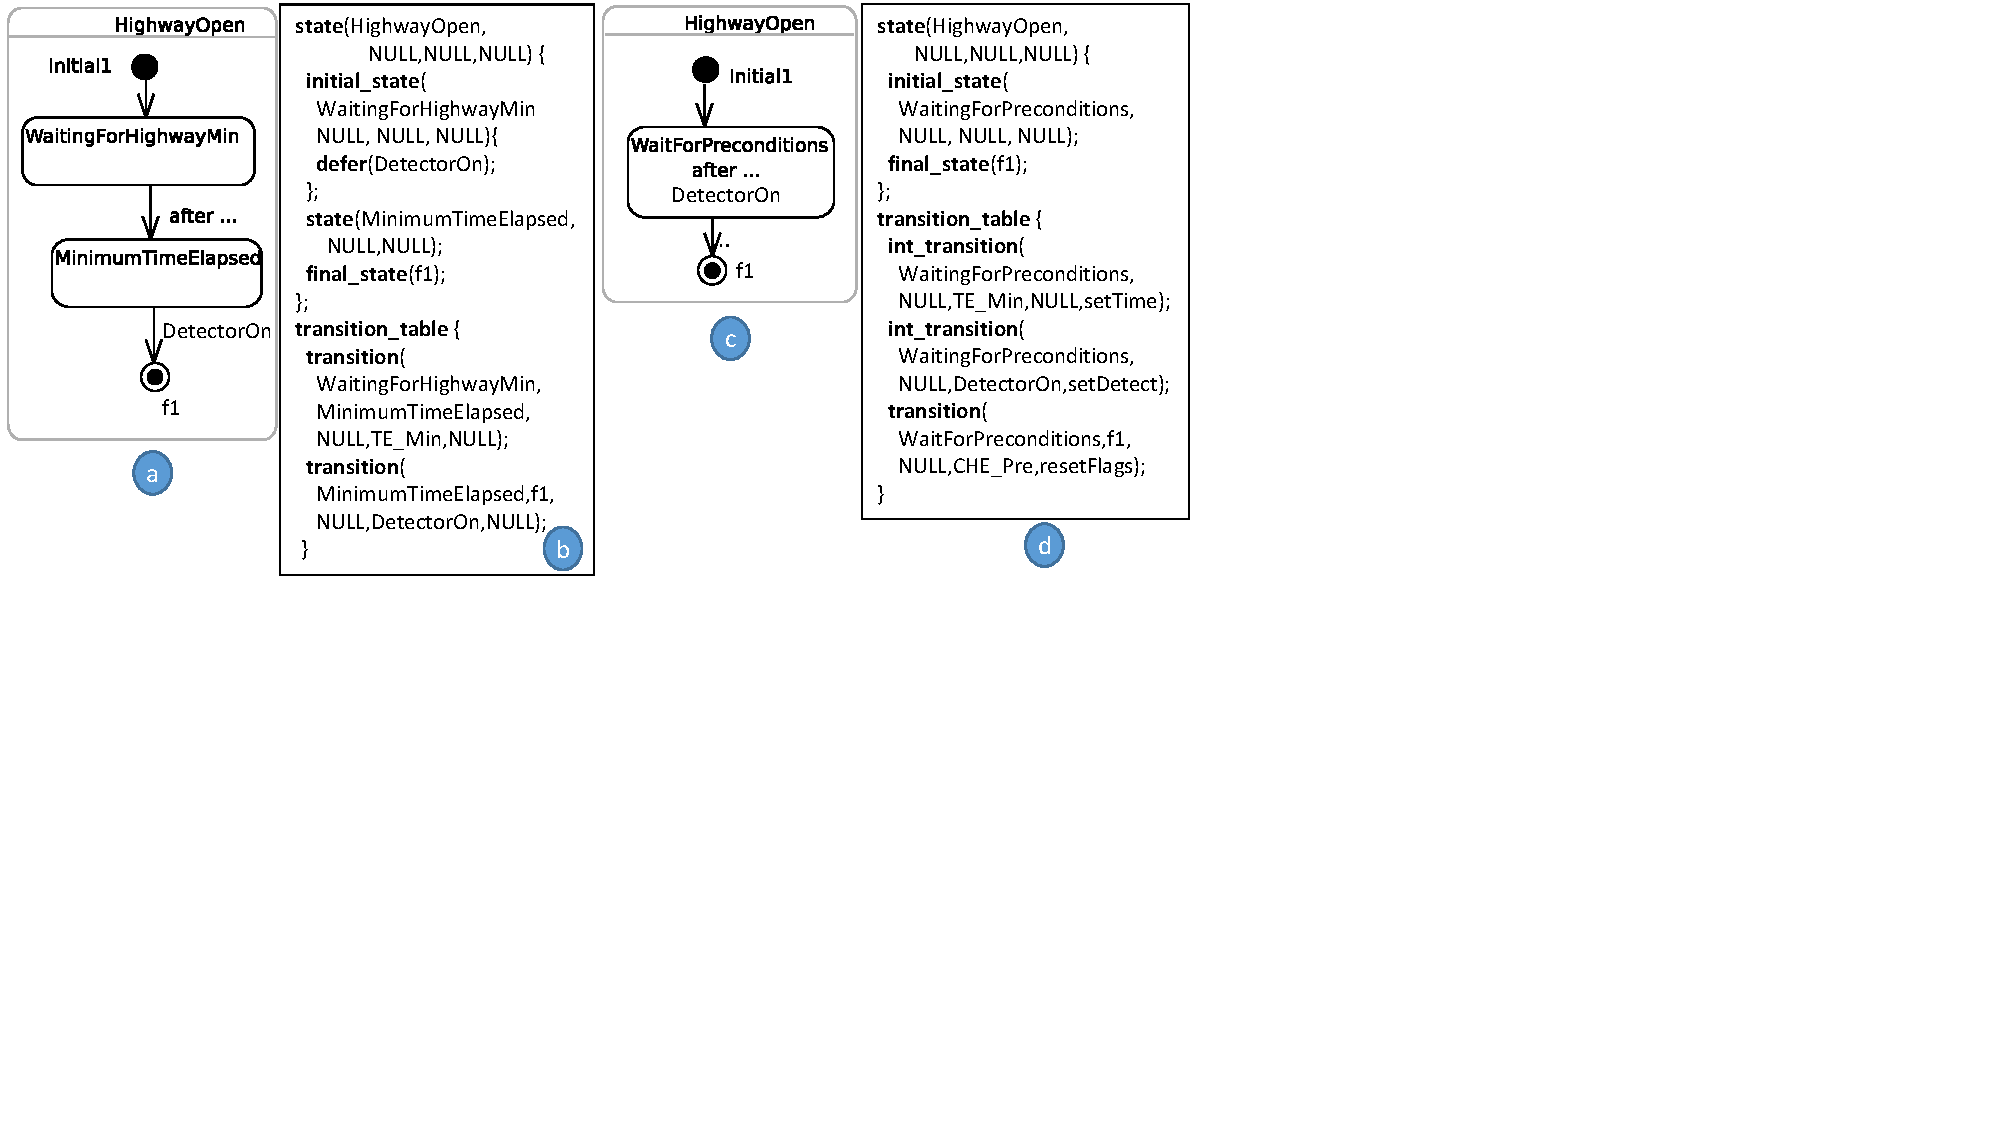
\includegraphics[clip, trim=0.0cm 9.3cm 12.7cm 0cm, width=\columnwidth]{figures/highwayopenalternatives}
	\caption{Alternative state machine design for the \ttt{HighwayOpen} state} 
	\label{fig:highwayopenalternatives}
\end{figure}

The architect creates the state machine for \ttt{Intersection} 
%since its behavior is complex and needs graphical tools to represent 
for better understanding.
For the programmer, he 
%is more familiar with C++. He 
develops the low-level behavior and creates the state machine for \ttt{TrafficLight} textually, from scratch.
These actors worked in parallel and synchronized their assignment after finishing.
The synchronization is realized by our previously presented process.
For simulation, we reuse the detector class developed in \cite{farmroadexample} to automatically generate \ttt{DetectorOn/DetectorOff} signals. 



%show the state machine and associated code

%show some comparison with the implementation of yasmine: line of code, binary size